%
% File acl2020.tex
%
%% Based on the style files for ACL 2020, which were
%% Based on the style files for ACL 2018, NAACL 2018/19, which were
%% Based on the style files for ACL-2015, with some improvements
%%  taken from the NAACL-2016 style
%% Based on the style files for ACL-2014, which were, in turn,
%% based on ACL-2013, ACL-2012, ACL-2011, ACL-2010, ACL-IJCNLP-2009,
%% EACL-2009, IJCNLP-2008...
%% Based on the style files for EACL 2006 by 
%%e.agirre@ehu.es or Sergi.Balari@uab.es
%% and that of ACL 08 by Joakim Nivre and Noah Smith

\documentclass[11pt,a4paper]{article}
\usepackage[hyperref]{acl2020}
\usepackage{times}
\usepackage{latexsym}
\renewcommand{\UrlFont}{\ttfamily\small}

% This is not strictly necessary, and may be commented out,
% but it will improve the layout of the manuscript,
% and will typically save some space.
\usepackage{microtype}

% custom
% \usepackage{fontspec}
% \setmainfont{Charis SIL}
% \usepackage{xeCJK}
% \setCJKmainfont{Noto Serif CJK KR}
% \usepackage[georgian]{babel}
\usepackage{booktabs}
\usepackage{graphicx}
\graphicspath{ {../images/} }

\aclfinalcopy % Uncomment this line for the final submission
%\def\aclpaperid{***} %  Enter the acl Paper ID here

%\setlength\titlebox{5cm}
% You can expand the titlebox if you need extra space
% to show all the authors. Please do not make the titlebox
% smaller than 5cm (the original size); we will check this
% in the camera-ready version and ask you to change it back.

\newcommand\BibTeX{B\textsc{ib}\TeX}

\title{Comparing Writing Systems with Multilingual Grapheme-to-Phoneme and Phoneme-to-Grapheme Conversion}

\author{Julen Etxaniz \\
  University of the Basque Country\\
  \texttt{\href{mailto:jetxaniz007@ikasle.ehu.eus}{jetxaniz007@ikasle.ehu.eus}}}

\date{}

\begin{document}
\maketitle
\begin{abstract}

\end{abstract}

\section{Introduction}

The orthographic depth of an alphabetic orthography indicates the degree to which a written language deviates from simple one-to-one grapheme (letter) to phoneme (sound) correspondence. 

Shallow (transparent) orthographies, also called phonemic orthographies, have a one-to-one relationship between its graphemes and phonemes, and the writing and reading of letters is very consistent. Spanish and Basque are examples of transparent orthographies.

In contrast, in deep (opaque) orthographies, the relationship is less direct, and the writer or reader must learn the arbitrarily irregular words. English and French are considered to have opaque orthographies.

Sequence-to-sequence models are very good at picking up on consistent patterns. Therefore, a seq2seq system should learn the regular writing systems much better than the irregular ones. That means that the performance of seq2seq models could be used as a measure of regularity of a writing system. The grapheme-to-phoneme (G2P) direction would suggest the difficulty of reading a language. Similarly, in the phoneme-to-grapheme (P2G) direction we would be looking at the inconsistencies of writing a language.

We use the transformer proposed in \citet{wu2021applying} to compare the orthographies of 10 languages: Armenian (Eastern), Bulgarian, Dutch, French, Georgian, Serbo-Croatian (Latin), Hungarian, Japanese (Hiragana), Korean and Vietnamese (Hanoi). We use same data of the medium-resource languages from the SIGMORPHON 2021 G2P task \cite{ashby-etal-2021-results}. We train a different model for each task and language.

The goal is not to build a perfect G2P and P2G system. Instead the goal is to build a translator which can indicate a degree of phonemic transparency and thus make it possible to rank orthographies. We do not have to translate a
sequence of words into another sequence of words. Our model only requires translating a single word. Therefore, We can consider G2P and P2G as two translation tasks and apply the transformer at character level.

\section{Related works}

Sequence-to-sequence (seq2seq) models have been proven to be very successful on language translation tasks. Recently, attention \cite{bahdanau2016neural}, transformers \cite{vaswani2017attention} and generative pre-training (GPT) \cite{Radford2018ImprovingLU} have improved the performance of seq2seq models. Applying the transformer to character-level transduction tasks such as G2P has been proved to be a good option \cite{wu2021applying}. It was one of the baselines in the SIGMORPHON 2020 G2P task \cite{gorman-etal-2020-sigmorphon}.

Many studies have discussed the transparency of orthographies based on the ease of reading and writing when learning a new language \cite{borleffs2017measuring}. However, there is not much work in NLP about measuring the level of transparency of an orthography. In an old work, three data-based algorithms were tested on three orthographies: Dutch, English and French \cite{bosch-1994-depth}.

In a recent work, a minimalist GPT implementation has been used to compare 17 orthographies \cite{marjou2021oteann} on the same G2P and P2G tasks. A unique multi-orthography model was trained to learn the writing and reading tasks on all languages at the same time. In other words, a single dataset containing samples of all studied orthographies was used.

On the one hand, the results show that Chinese, French, English and Russian are the most opaque regarding writing. English and Dutch are the most opaque regarding reading. 

On the other hand, they indicate that Esperanto, Arabic, Finnish, Korean, Serbo-Croatian and Turkish are very shallow both to read and to write. Italian, Breton, German, Portuguese and Spanish are shallow to read and to write.

\section{Material and methods}

All the code and data is available on GitHub\footnote{\url{https://github.com/juletx/writing-systems}}.

\subsection{Data}

\begin{table*}[h]
\centering
\begin{tabular}{llllll}
\toprule
               Language &       Code & Graphemes & Phonemes & Mean Gra & Mean Pho \\
\midrule
     Armenian (Eastern) &      arm\_e &               38 &              41 &              7.09 &                7 \\
              Bulgarian &        bul &               29 &              45 &              8.44 &             8.64 \\
                  Dutch &        dut &               30 &              45 &              7.71 &             6.99 \\
                 French &        fre &               37 &              37 &              7.52 &             5.75 \\
               Georgian &        geo &               33 &              33 &              7.74 &             7.74 \\
 Serbo-Croatian (Latin) &   hbs\_latn &               27 &              61 &              7.47 &             7.36 \\
              Hungarian &        hun &               34 &              61 &              7.65 &             7.18 \\
    Japanese (Hiragana) &   jpn\_hira &               76 &              64 &              4.21 &             6.56 \\
                 Korean &        kor &              559 &              60 &              2.58 &             6.54 \\
     Vietnamese (Hanoi) &  vie\_hanoi &               89 &              49 &              5.81 &             7.51 \\
\midrule
                Average &    average &             95.2 &            49.6 &              6.62 &             7.13 \\
\bottomrule
\end{tabular}
\end{table*}

\subsection{Preprocessing}

\subsection{Training}

The training process was monitored using TensorBoard\footnote{\url{https://tensorboard.dev/experiment/mcrHkdndR0ySobcxV1UxVA}}.

\subsection{Evaluation}

The metric used to rank systems is word error rate (WER), the percentage of words for which the predicted sequence does not match the gold sequence. The average WER was also calculated for each task. This is the same metric that was used in SIGMORPHON 2021 Task 1. The evaluation was performed using the scripts provided in that task.

\subsection{Baseline}

The baseline for the SIGMORPHON 2021 G2P task is a neural transducer system using an imitation learning paradigm \cite{makarov-clematide-2018-imitation}. Alignments are computed using ten iterations of expectation maximization, and the imitation learning policy is trained for up to sixty epochs (with a patience of twelve) using the Adadelta optimizer. A beam of size of four is used for prediction. Final predictions are produced by a majority-vote ten-component ensemble.

\section{Results}

\subsection{Comparison with baseline}

The G2P results are compared with the baseline results on the dev and test sets in Table \ref{tab:baseline} and Figure \ref{fig:baseline}. The results are worse in all languages but the ranking between languages is maintained. As we said before, our aim is not to get perfect results, so our model is good enough for our aim.

\begin{table*}[h]
\centering
\begin{tabular}{lrrrr}
\toprule
      Code &  Baseline Dev &   Dev &  Baseline Test &   Test \\
\midrule
     arm\_e &          4.50 &   6.5 &           7.00 &   8.90 \\
       bul &          8.30 &  14.9 &          18.30 &  20.10 \\
       dut &         10.80 &  12.0 &          14.70 &  16.90 \\
       fre &          7.40 &   9.5 &           8.50 &  10.20 \\
       geo &          0.00 &   0.3 &           0.00 &   0.10 \\
  hbs\_latn &         34.70 &  49.2 &          32.10 &  47.70 \\
       hun &          1.50 &   2.8 &           1.80 &   1.90 \\
  jpn\_hira &          6.20 &   8.4 &           5.20 &   8.50 \\
       kor &         18.40 &  33.4 &          16.30 &  30.20 \\
 vie\_hanoi &          1.30 &   4.0 &           2.50 &   6.00 \\
\midrule
   average &          9.31 &  14.1 &          10.64 &  15.05 \\
\bottomrule
\end{tabular}
\caption{Comparison of our G2P results with the baseline}
\label{tab:baseline}
\end{table*}

\begin{figure}[h]
    \centering
    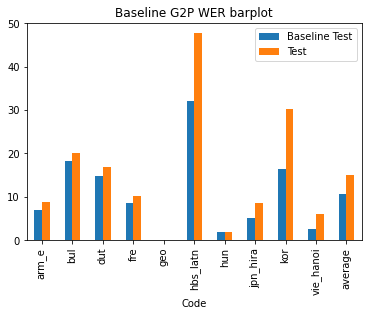
\includegraphics[width=\linewidth]{g2p_baseline.png}
    \caption{Comparison of our G2P results with the baseline}
    \label{fig:baseline}
\end{figure}

\subsection{Comparison between languages}

\begin{table*}[h]
\centering
\begin{tabular}{lrrrrrr}
\toprule
      Code &  G2P Train &  G2P Dev &  G2P Test &  P2G Train &  P2G Dev &  P2G Test \\
\midrule
     arm\_e &       1.16 &      6.5 &      8.90 &       0.57 &     4.40 &      5.70 \\
       bul &       0.34 &     14.9 &     20.10 &      16.25 &    19.70 &     27.30 \\
       dut &       2.59 &     12.0 &     16.90 &       2.67 &    18.00 &     23.00 \\
       fre &       2.04 &      9.5 &     10.20 &      32.96 &    53.50 &     54.00 \\
       geo &       0.06 &      0.3 &      0.10 &       0.12 &     0.30 &      0.50 \\
  hbs\_latn &      22.56 &     49.2 &     47.70 &       0.09 &     0.20 &      0.60 \\
       hun &       0.64 &      2.8 &      1.90 &       0.84 &     6.20 &      4.80 \\
  jpn\_hira &       2.74 &      8.4 &      8.50 &       0.59 &     2.40 &      3.90 \\
       kor &      19.27 &     33.4 &     30.20 &      11.84 &    22.80 &     22.10 \\
 vie\_hanoi &       0.44 &      4.0 &      6.00 &       5.35 &    15.00 &     16.30 \\
 \midrule
   average &       5.18 &     14.1 &     15.05 &       7.13 &    14.25 &     15.82 \\
\bottomrule
\end{tabular}
\end{table*}


\bibliography{writing_systems}
\bibliographystyle{acl_natbib}

\end{document}
